% 3.3.4 Construcción de las tarjetas principales (T4): estado del tablero y API + interfaz por tarjeta.
% Sin fechas (solo en 3.5). Capturas con datos ficticios en img/Objetivo3/.

\subsubsection{Construcción: tarjetas del sistema}

La construcción siguió las tarjetas del plan (Tabla~\ref{tab:ob2_tarjetas}) con una sola tarjeta en desarrollo. El tablero se gestionó en Planka, de código abierto. Cada tarjeta agrupa en una lista las tareas de la API y de la interfaz web que se construyeron a la vez, y en otra sus pruebas (Figura~\ref{fig:ob3_tarjeta_detalle}). La Tabla~\ref{tab:ob3_tarjetas} resume el estado final, y los apartados siguientes detallan las tarjetas que atienden los puntos críticos del Objetivo 1.

\begingroup
\fontsize{9}{11}\selectfont
\renewcommand{\arraystretch}{1.2}
\setlength{\LTpre}{0pt}\setlength{\LTpost}{6pt}
\setlength{\tabcolsep}{4pt}
\begin{xltabular}{\linewidth}{|>{\raggedright\arraybackslash}X|>{\raggedright\arraybackslash}p{4.4cm}|}
\caption{Estado final de las tarjetas del tablero}
\label{tab:ob3_tarjetas} \\
\hline
\textbf{Tarjeta} & \textbf{Estado} \\ \hline
\endfirsthead
\hline
\textbf{Tarjeta} & \textbf{Estado} \\ \hline
\endhead
0. Base del proyecto: estructura, base de datos y pruebas & Completada \\ \hline
1 a 10. Identidad, pacientes y profesionales, historia clínica, agenda, atención, odontograma, tratamientos, recetas, cobros y auditoría & Completadas \\ \hline
11 a 13. Agente: núcleo, agendamiento e interpretación del texto libre & Completadas \\ \hline
14. Agente: recordatorios & No implementada (Debería); retirada del tablero \\ \hline
15. Respaldos y exportación & \textit{[Respaldos completados; falta la exportación]} \\ \hline
\multicolumn{2}{|l|}{\cellcolor{gray!10}\textbf{Tarjetas añadidas durante la construcción}} \\ \hline
Formulario 033: vista, impresión e historial inmediato & Completada \\ \hline
Funciones del director: usuarios, profesionales, catálogos y estadísticas & Completada \\ \hline
Ajustes del prototipo (Tabla~\ref{tab:ob3_ajustes}) & Completada \\ \hline
Despliegue en el servidor e integración continua & Completada \\ \hline
\end{xltabular}
\endgroup

\begin{figure}[H]
\centering
\IfFileExists{img/Objetivo3/Ob3_Tarjeta_Agenda.png}{\includegraphics[width=0.8\linewidth]{img/Objetivo3/Ob3_Tarjeta_Agenda.png}}{\fbox{\parbox{0.9\linewidth}{\centering Pendiente: img/Objetivo3/Ob3\_Tarjeta\_Agenda.png}}}
\caption{Tarjeta 4 del tablero, con su trazabilidad, sus tareas y sus pruebas}
\label{fig:ob3_tarjeta_detalle}
\end{figure}

\paragraph{Identidad y roles}

\textbf{API.} El inicio de sesión devuelve un token firmado (JWT) con los permisos del usuario; cada operación exige su permiso y las contraseñas se guardan cifradas (RNF01, BN4). \textbf{Interfaz.} El perfil se deriva del rol: cada perfil tiene su menú y sus rutas, y los botones se muestran según el permiso (Figura~\ref{fig:ob3_login}).

\begin{figure}[H]
\centering
\IfFileExists{img/Objetivo3/Ob3_Login_Perfiles.png}{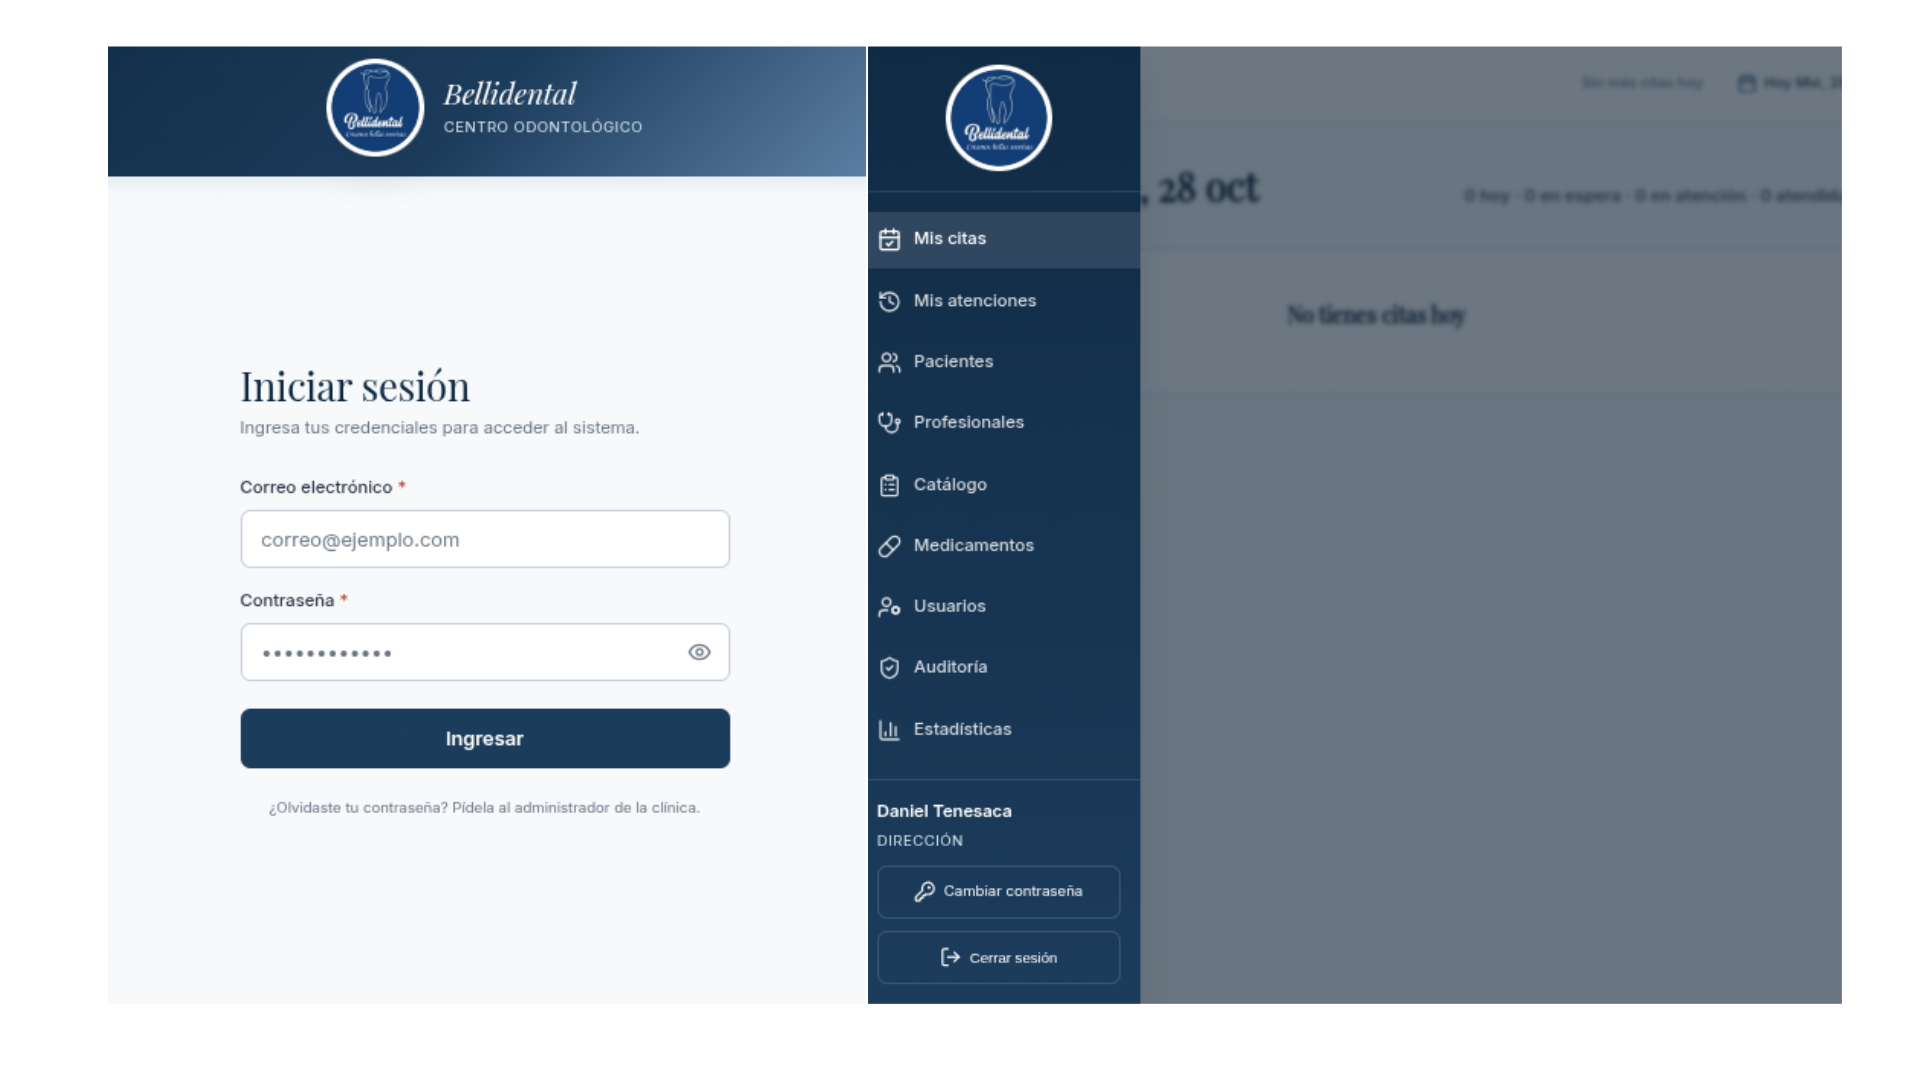
\includegraphics[width=\linewidth]{img/Objetivo3/Ob3_Login_Perfiles.png}}{\fbox{\parbox{0.9\linewidth}{\centering Pendiente: img/Objetivo3/Ob3\_Login\_Perfiles.png}}}
\caption{Inicio de sesión y menú por perfil}
\label{fig:ob3_login}
\end{figure}

\paragraph{Agenda sin cruces}

\textbf{API.} La disponibilidad es el horario efectivo del profesional menos sus citas activas, en bloques de 15 min y con duración de 15 a 240 min. Los estados siguen el diseño (Figura~\ref{fig:ob2_estados_cita}); un cruce lo rechaza la restricción de exclusión (Figura~\ref{fig:ob3_exclude}) y la API lo devuelve como conflicto (RF07). \textbf{Interfaz.} La agenda del día muestra una columna por profesional con su color, el origen de cada cita y el aviso de rechazo ante un cruce (Figura~\ref{fig:ob3_agenda}).

\begin{figure}[H]
\centering
\IfFileExists{img/Objetivo3/Ob3_Agenda.png}{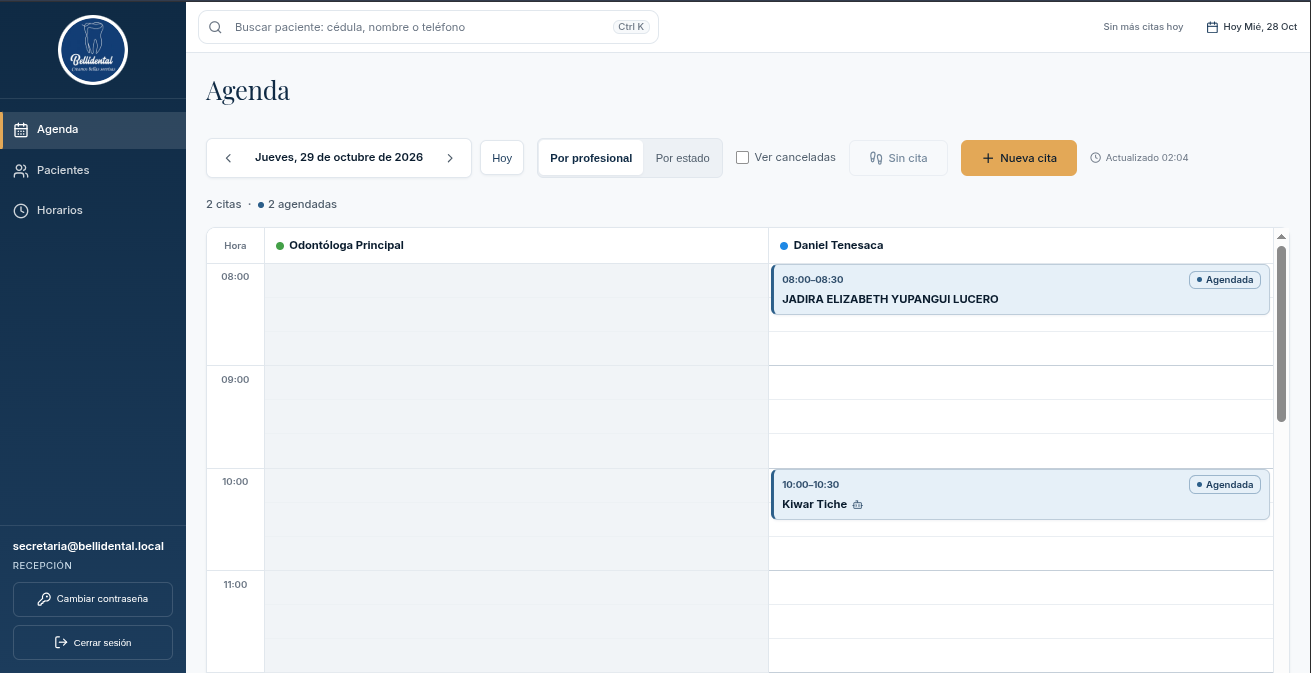
\includegraphics[width=\linewidth]{img/Objetivo3/Ob3_Agenda.png}}{\fbox{\parbox{0.9\linewidth}{\centering Pendiente: img/Objetivo3/Ob3\_Agenda.png}}}
\caption{Agenda del día de la secretaria}
\label{fig:ob3_agenda}
\end{figure}

\paragraph{Atención clínica y odontograma}

\textbf{API.} Solo el odontólogo abre la atención, tras el registro de llegada; cerrarla exige el motivo y al menos un diagnóstico, y la cita pasa a atendida. El CIE-10 se busca por código o por similitud de texto, y cada hallazgo se registra por pieza y cara como pendiente o realizado. Las correcciones anulan el registro y crean otro (RF01 a RF03; BN1, BN3, BN5). \textbf{Interfaz.} Una sola pantalla reúne la cabecera clínica, los antecedentes, los diagnósticos y el odontograma, que se marca en dos clics (Figura~\ref{fig:ob3_atencion}).

\begin{figure}[H]
\centering
\IfFileExists{img/Objetivo3/Ob3_Atencion.png}{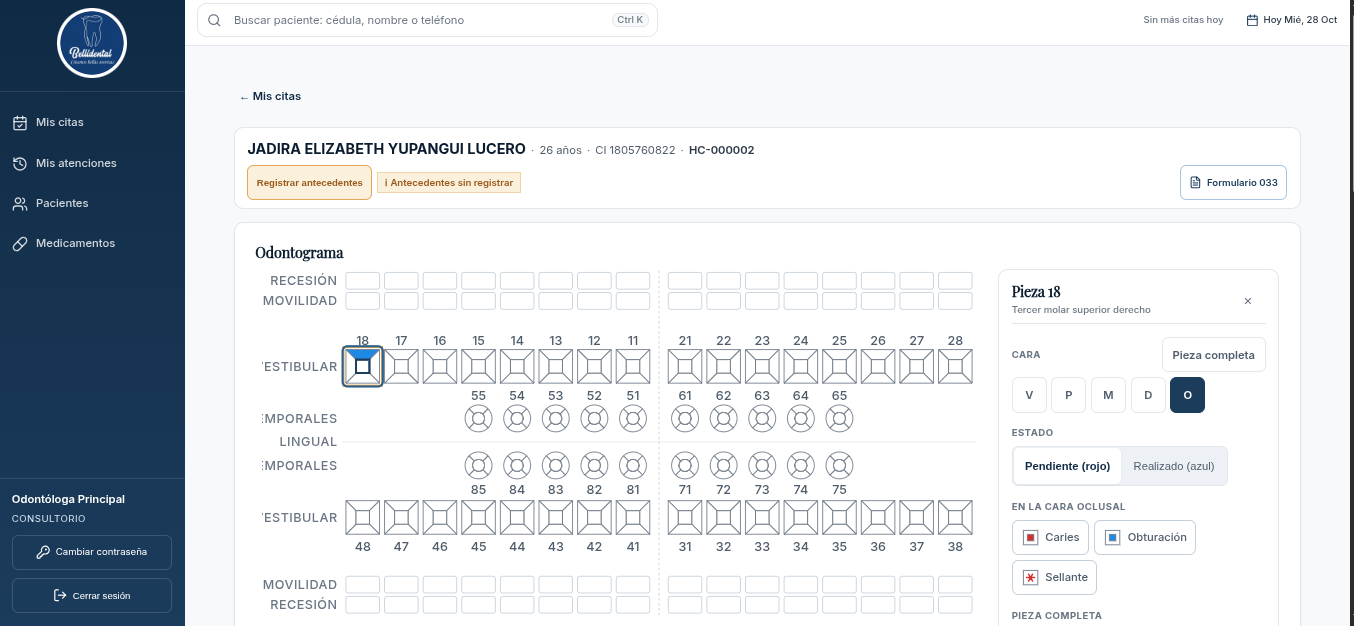
\includegraphics[width=\linewidth]{img/Objetivo3/Ob3_Atencion.png}}{\fbox{\parbox{0.9\linewidth}{\centering Pendiente: img/Objetivo3/Ob3\_Atencion.png}}}
\caption{Atención con antecedentes, diagnósticos y odontograma}
\label{fig:ob3_atencion}
\end{figure}

\paragraph{Tratamientos, receta y Formulario 033}

\textbf{API.} El tratamiento se elige del catálogo con su precio base, editable; si se liga a un hallazgo pendiente, este pasa a realizado. La receta nace como borrador y, al emitirse, queda inmutable y se genera en PDF con la leyenda de confidencialidad y el espacio para la firma (RF04, RF05). \textbf{Interfaz.} Tratamientos y receta se registran en un panel lateral, con posologías predefinidas (Figura~\ref{fig:ob3_receta}); el Formulario 033 se compone de lo registrado y se imprime en el formato del MSP (Figura~\ref{fig:ob3_form033}), lo que elimina la transcripción de la Etapa 2 (BN1, BN2). Su sección 12 reúne todas las sesiones del paciente y sirve de historial inmediato desde cualquier atención (RF06).

\begin{figure}[H]
\centering
\IfFileExists{img/Objetivo3/Ob3_Receta.png}{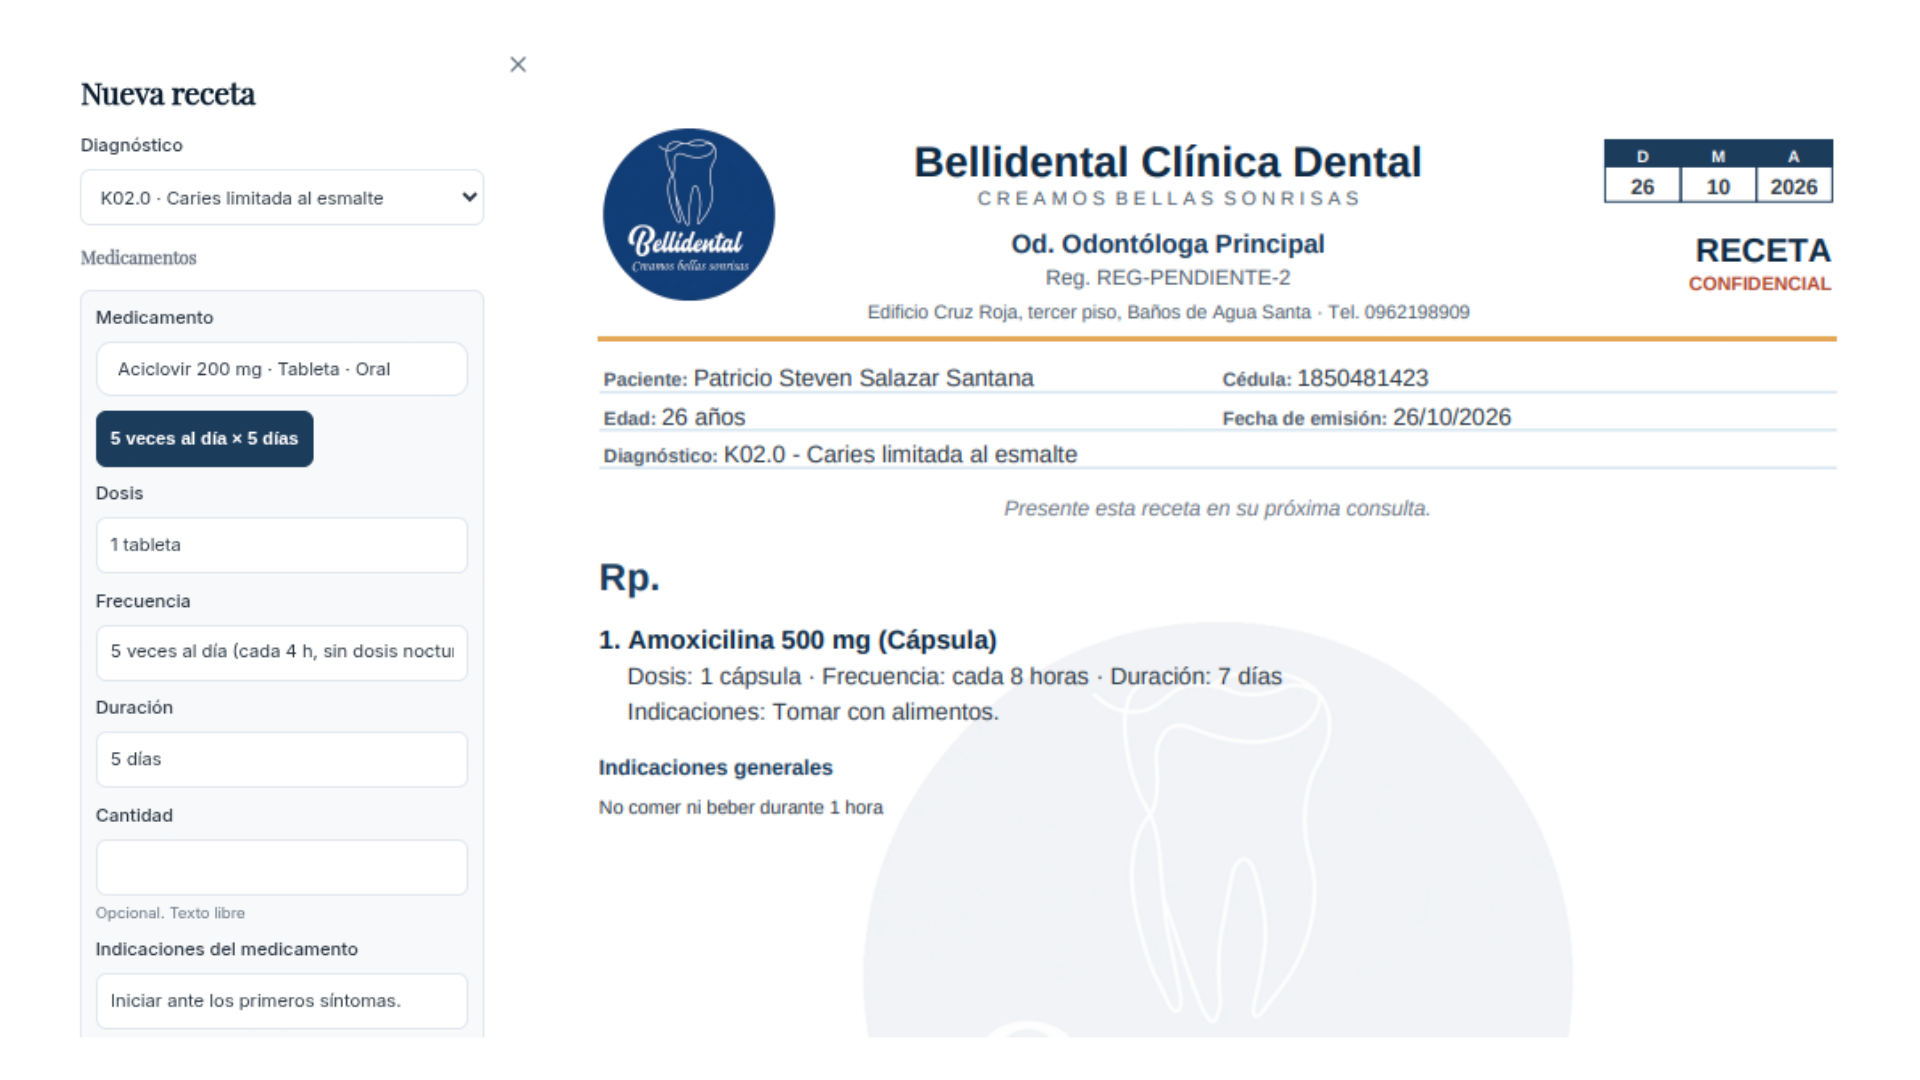
\includegraphics[width=\linewidth]{img/Objetivo3/Ob3_Receta.png}}{\fbox{\parbox{0.9\linewidth}{\centering Pendiente: img/Objetivo3/Ob3\_Receta.png}}}
\caption{Tratamientos de la atención y receta emitida}
\label{fig:ob3_receta}
\end{figure}

\begin{figure}[H]
\centering
\IfFileExists{img/Objetivo3/Ob3_Form033.png}{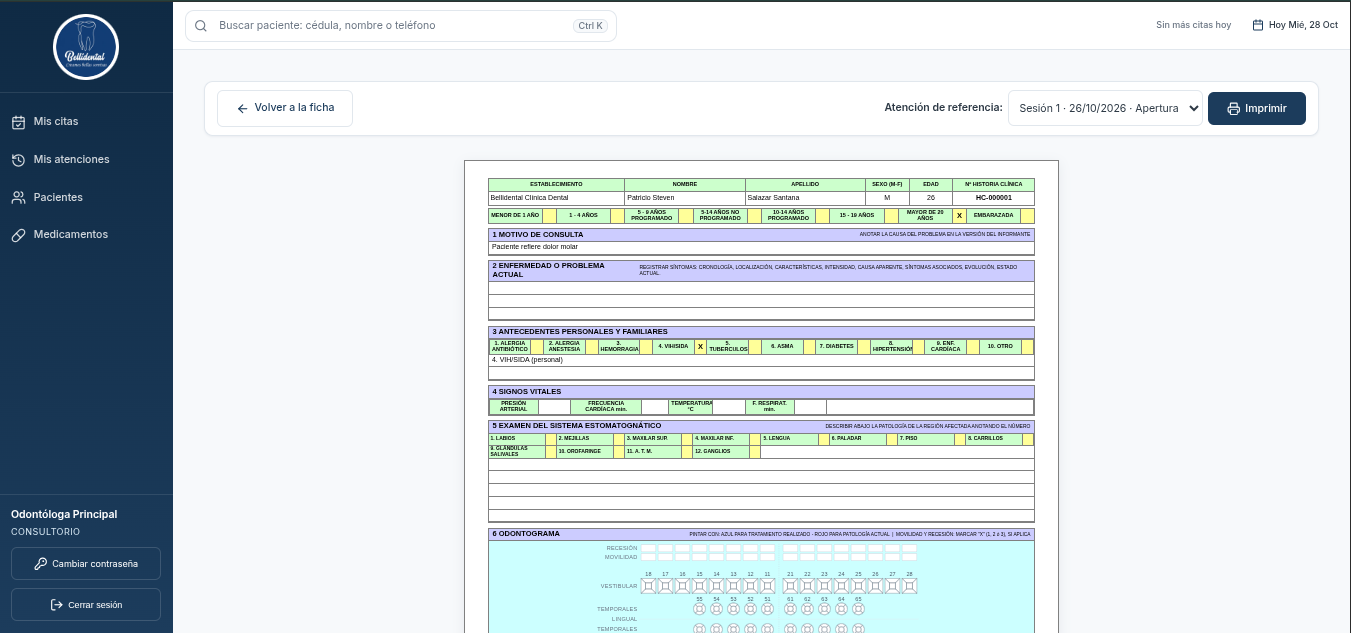
\includegraphics[width=\linewidth]{img/Objetivo3/Ob3_Form033.png}}{\fbox{\parbox{0.9\linewidth}{\centering Pendiente: img/Objetivo3/Ob3\_Form033.png}}}
\caption{Formulario 033 generado por el sistema}
\label{fig:ob3_form033}
\end{figure}

\paragraph{Cobros}

\textbf{API.} El saldo se calcula con los tratamientos y los pagos vigentes; cada abono genera un comprobante numerado en PDF, y un pago solo se anula con motivo (RF08). \textbf{Interfaz.} La ficha de recepción muestra el estado de cuenta por sesión, sin diagnósticos, y registra el abono (Figura~\ref{fig:ob3_cobro}; RNF01).

\begin{figure}[H]
\centering
\IfFileExists{img/Objetivo3/Ob3_Cobro.png}{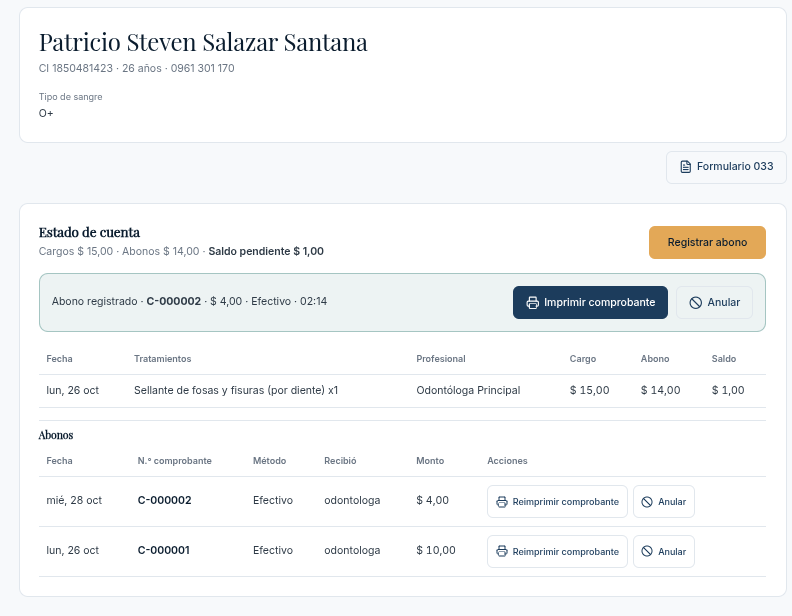
\includegraphics[width=\linewidth]{img/Objetivo3/Ob3_Cobro.png}}{\fbox{\parbox{0.9\linewidth}{\centering Pendiente: img/Objetivo3/Ob3\_Cobro.png}}}
\caption{Ficha de recepción con estado de cuenta y registro del abono}
\label{fig:ob3_cobro}
\end{figure}

\paragraph{Funciones del director y auditoría}

\textbf{API.} Cada cambio en los registros auditados guarda una revisión con usuario y fecha, consultable por registro (RNF02, BN4). \textbf{Interfaz.} El director administra usuarios, profesionales y catálogos, consulta las estadísticas de la clínica y abre el historial de cambios desde el paciente o la atención (Figura~\ref{fig:ob3_director}).

\begin{figure}[H]
\centering
\IfFileExists{img/Objetivo3/Ob3_Director.png}{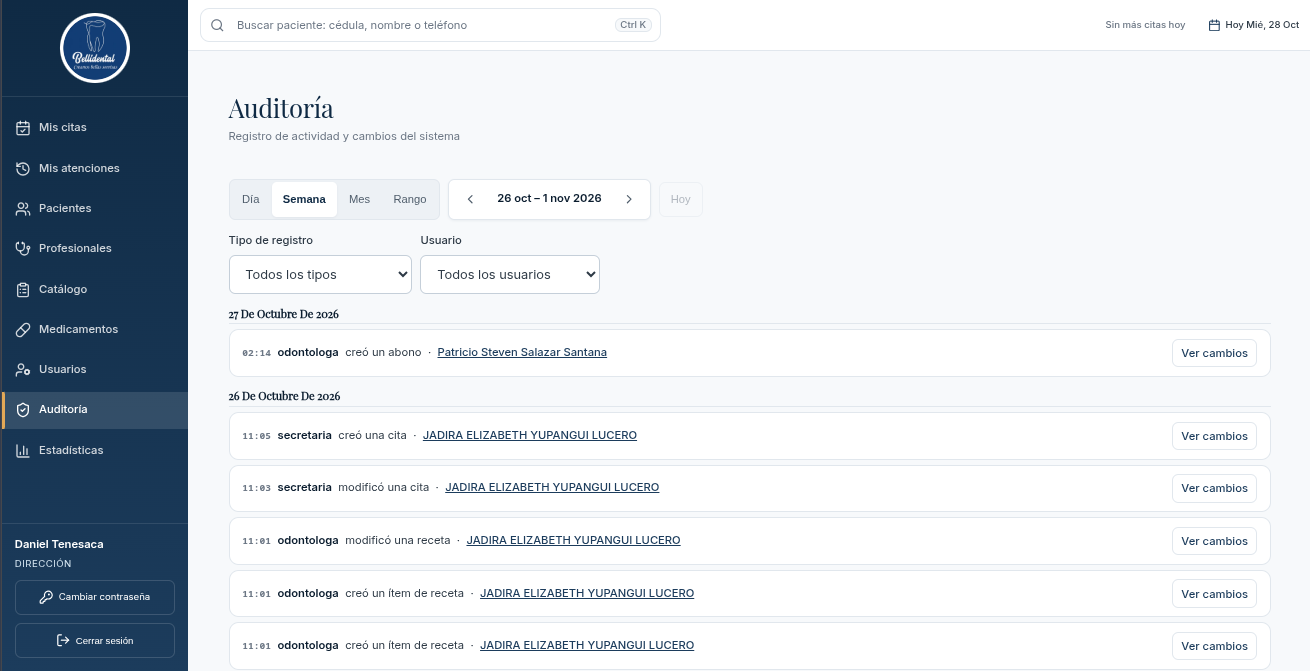
\includegraphics[width=\linewidth]{img/Objetivo3/Ob3_Director.png}}{\fbox{\parbox{0.9\linewidth}{\centering Pendiente: img/Objetivo3/Ob3\_Director.png}}}
\caption{Estadísticas e historial de cambios del director}
\label{fig:ob3_director}
\end{figure}
